\documentclass{standalone}

\usepackage[english]{babel}
\usepackage[linesnumbered, ruled, vlined]{algorithm2e}

\usepackage{caption}

% to create listings

\usepackage{listings, lstautogobble}
\lstset{
  autogobble=true,
  frame=single,
}

\lstdefinelanguage{coq}[Objective]{Caml}{
  morekeywords={Structure, Definition, Inductive, list, return},
  sensitive=true
}

% to define font size

\usepackage{ulem}
\usepackage{moresize}
\usepackage{anyfontsize}

% to use tikz and its libraries

\usepackage{tikz-timing}
\usepackage{tikz}

\usetikzlibrary{backgrounds}
\usetikzlibrary{positioning, calc, arrows, shapes, automata, petri, patterns}

% to use tikzmark, to place and refer to marks outside the current figure

\tikzset{every picture/.style={remember picture}}

% styles for transitions

\tikzset{transition/.append style={fill=black!20, thick}}
\tikzset{transition/.append style={fill=black!20, thick}}

% styles for test and inhib arcs.

\tikzstyle{test}=[pre, *-]
\tikzstyle{inhib}=[pre, o-]

% to use colors

\usepackage{xcolor}

%%%%%%%%%%%%%%%%%%%%%%%%%%%%%%%%%%%%%%%%%%%%%%%%%%
%                  BEGIN DOCUMENT                %
%%%%%%%%%%%%%%%%%%%%%%%%%%%%%%%%%%%%%%%%%%%%%%%%%%

\begin{document}

\begin{tikzpicture}

  \node (pn1) {
    \begin{tikzpicture}
      \node[place, tokens=2] (p0) [label={above:$p_0$}] {};
      
      \node[transition, anchor=north east] (t0) at ($(p0.south west)-(.5,.5)$) [label={left:\textcolor{red}{$t_0$}}] {}
      edge[pre, bend left] (p0);

      \node[transition, anchor=north west] (t2) at ($(p0.south east)+(.5,-.5)$) [label={right:$t_2$}] {}
      edge[pre, bend right] (p0);

      \node[transition] (t1) at ($(t0)!.5!(t2)$) [label={left:$t_1$}] {}
      edge[pre] (p0);
      \node[anchor=west] at ($(t1.east)$) {\textcolor{red}{$c_0$}};

      \draw ($(t0.south)$) edge[bend right, dotted, ->] ($(t1.south west)$);
      \draw ($(t1.south)$) edge[bend right, dotted, ->] ($(t2.south west)$);
    \end{tikzpicture}    
  };

  \node[anchor=north, draw, circle, inner sep=1pt] at (pn1.south) {1};

  \node (pn2) at ($(pn1.east)+(2,0)$) {
    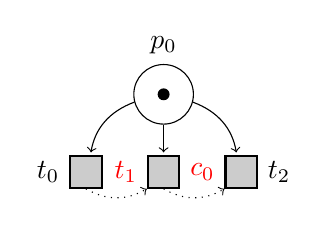
\begin{tikzpicture}
      \node[place, tokens=1] (p0) [label={above:$p_0$}] {};
      
      \node[transition, anchor=north east] (t0) at ($(p0.south west)-(.5,.5)$) [label={left:$t_0$}] {}
      edge[pre, bend left] (p0);

      \node[transition, anchor=north west] (t2) at ($(p0.south east)+(.5,-.5)$) [label={right:$t_2$}] {}
      edge[pre, bend right] (p0);

      \node[transition] (t1) at ($(t0)!.5!(t2)$) [label={left:\textcolor{red}{$t_1$}}] {}
      edge[pre] (p0);
      \node[anchor=west] at ($(t1.east)$) {\textcolor{red}{$c_0$}};
      \draw ($(t0.south)$) edge[bend right, dotted, ->] ($(t1.south west)$);
      \draw ($(t1.south)$) edge[bend right, dotted, ->] ($(t2.south west)$);
    \end{tikzpicture}
    
  };

  \node[anchor=north, draw, circle, inner sep=1pt] at (pn2.south) {2};

  \node (pn3) at ($(pn2.east)+(2,0)$) {
    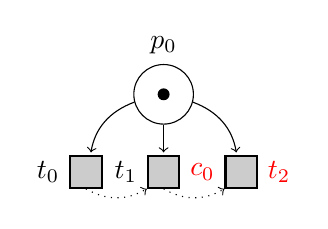
\begin{tikzpicture}
      \node[place, tokens=1] (p0) [label={above:$p_0$}] {};
      
      \node[transition, anchor=north east] (t0) at ($(p0.south west)-(.5,.5)$) [label={left:$t_0$}] {}
      edge[pre, bend left] (p0);

      \node[transition, anchor=north west] (t2) at ($(p0.south east)+(.5,-.5)$) [label={right:\textcolor{red}{$t_2$}}] {}
      edge[pre, bend right] (p0);

      \node[transition] (t1) at ($(t0)!.5!(t2)$) [label={left:$t_1$}] {}
      edge[pre] (p0);
      \node[anchor=west] at ($(t1.east)$) {\textcolor{red}{$c_0$}};      
      \draw ($(t0.south)$) edge[bend right, dotted, ->] ($(t1.south west)$);
      \draw ($(t1.south)$) edge[bend right, dotted, ->] ($(t2.south west)$);
    \end{tikzpicture}
  };

  \node[anchor=north, draw, circle, inner sep=1pt] at (pn3.south) {3};
  
\end{tikzpicture}

\end{document}
%%% Local Variables:
%%% mode: latex
%%% TeX-master: t
%%% End:
